\section{Sensing Methods for Lubrication Condition Monitoring}
\label{sec:sensing}

Online sensing methods for collecting data informative of the lubrication condition in ball bearings can be categorised along two independent axes. A method is \textbf{active} if it supplies external energy into the bearing system in order to probe its response; it is \textbf{passive} if it relies solely on signals inherently generated by the bearing under operation. A method is \textbf{invasive} if it requires unobstructed line-of-sight into the bearing, direct physical contact with the lubricant, mounting inside the bearing, structural modifications, or physical extraction of lubricant samples; it is \textbf{non-invasive} if none of these requirements apply.

These two axes define four categories illustrated in Figure~\ref{fig:taxonomy}: active/invasive (e.g., optical interferometry, ultrasonic reflectometry), active/non-invasive (e.g., external ultrasonic pulse-echo with external transducer), passive/invasive (e.g., direct lubricant sampling), and passive/non-invasive (e.g., acoustic emission, vibration, thermal monitoring). The passive/non-invasive category is of particular industrial relevance because its methods can be applied to bearings in service without modification and without interrupting operation. The present review covers all four categories for completeness but gives greatest depth to the passive/non-invasive methods.

\begin{figure}[H]
\centering
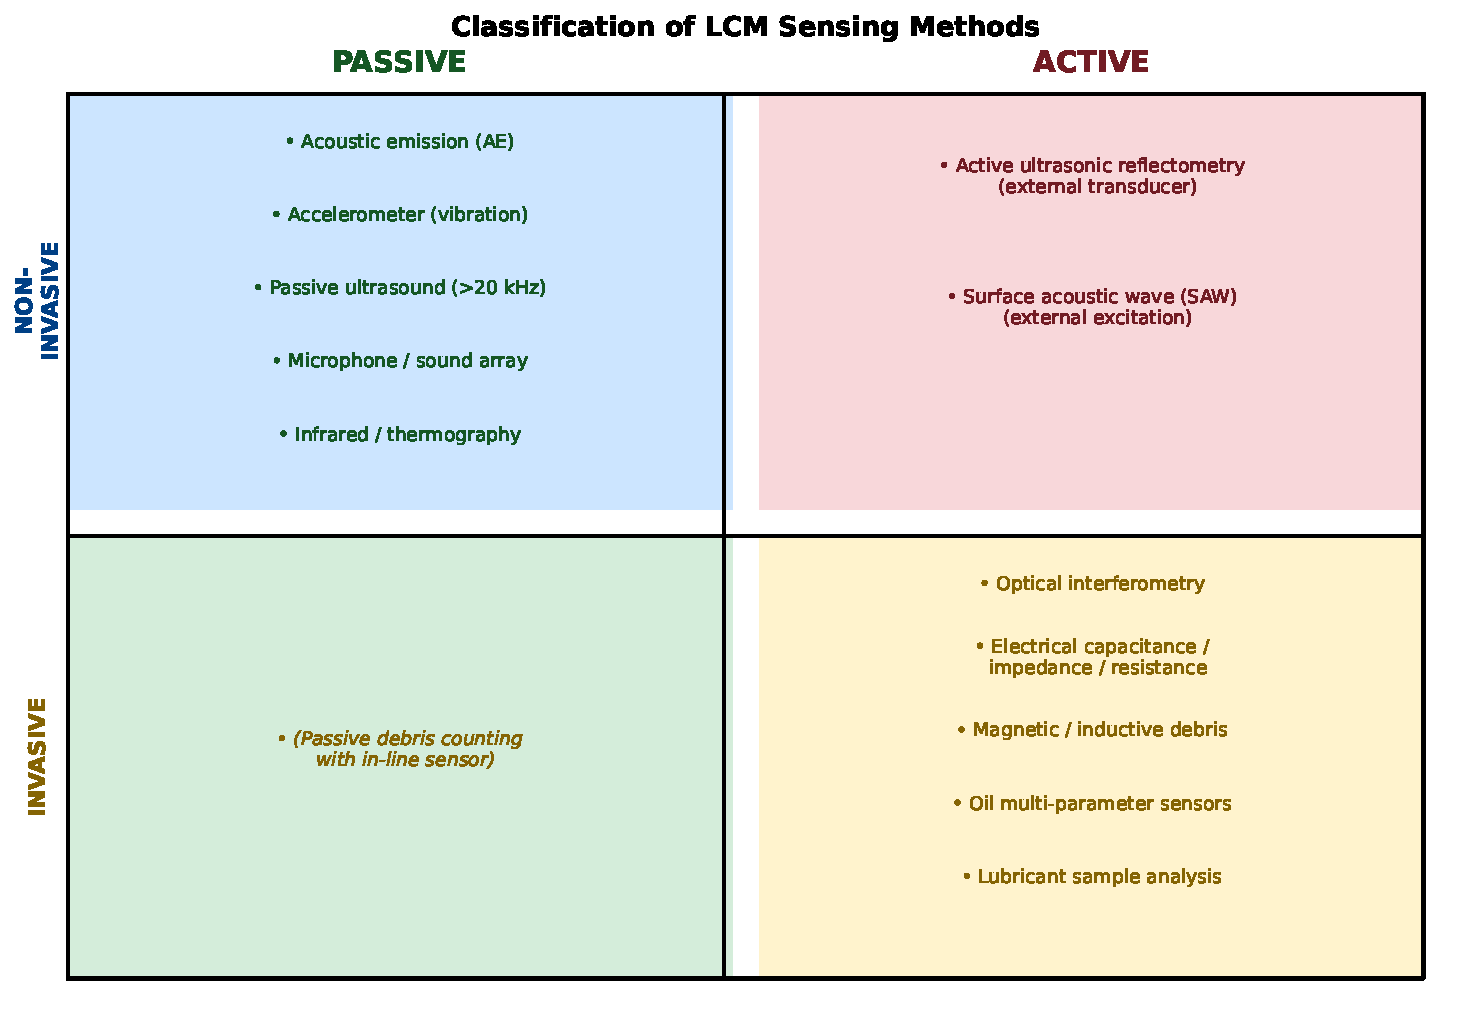
\includegraphics[width=0.72\textwidth]{figures/sensing_taxonomy.pdf}
\caption{Classification of sensing methods for lubrication condition monitoring along two independent axes: active vs.\ passive signal acquisition, and invasive vs.\ non-invasive installation requirements. Representative sensing modalities are placed in each quadrant.}
\label{fig:taxonomy}
\end{figure}

\noindent The subsections below describe each sensing modality with a standardised structure: (i) physical principle, (ii) what lubrication information it is sensitive to, and (iii) installation and operational characteristics. Signal processing methods are treated in depth in Section~\ref{sec:sp}.

% ─────────────────────────────────────────────────────────────────────────────
\subsection{Passive and Non-Invasive Methods}
\label{subsec:passive_noninv}

\subsubsection{Acoustic Emission}
\label{subsubsec:ae}
Acoustic emission (AE) refers to transient, high-frequency elastic stress waves -- typically in the range 20\,kHz to 1\,MHz -- spontaneously generated within the bearing material and contact interfaces as a result of tribological processes. These processes include asperity contact and micro-fracture under inadequate lubrication, crack initiation and propagation under cyclic contact stress, wear particle generation, and frictional energy release at rolling and sliding contacts \cite{hou_-situ_2025,delft_university_of_technology_tu_delft_influence_2024,scheeren_acoustic_2024}. AE sensors are piezoelectric transducers mounted on the bearing housing, raceway, or an adjacent structural component and capture these stress waves non-invasively.

AE is sensitive to the lubrication regime: as the specific film thickness $\Lambda$ decreases from EHL toward boundary lubrication, asperity contacts increase in frequency and severity, generating more AE energy. Cornel et al.\ \cite{cornel_condition_2021} demonstrate a direct inverse correlation between AE amplitude and $\Lambda$ in cylindrical roller bearings under controlled lubrication conditions. Hou and Zhang \cite{hou_-situ_2025} show that AE amplitude centre and energy centre in thrust ball bearings map onto distinct lubrication regime clusters and can be used to estimate $\Lambda$ with 89.3\% accuracy. Miettinen et al.\ \cite{miettinen_analysis_2001} show that the pulse count rate increases monotonically with grease starvation and differentiates among ten grease compositions. An important exception to the monotonic amplitude-lubrication relationship is the non-monotonic energy response observed by Hou and Zhang, in which transitioning from dry contact to low-viscosity lubrication initially \textit{decreases} AE energy before it rises again with increasing viscosity due to viscous damping forces on the bearing ring. This highlights that AE-lubrication relationships are configuration-specific and require calibration.

AE consistently provides earlier detection of sub-surface damage and lubrication degradation than conventional vibration sensors. Cornel et al.\ \cite{cornel_condition_2021} report approximately 50\% earlier detection of sub-surface damage deviations compared to vibration RMS. Yoshioka and Shimizu \cite{yoshioka_monitoring_2009} find that demodulated AE mean changes before vibration RMS in conditions without significant fretting corrosion. The primary practical challenge is the large data volume generated by continuous AE acquisition at the required sampling rates ($>$500\,kHz), which most studies address through windowed statistical features, interval sampling, or event-triggered recording.

Multi-technique comparison of passive sensing methods for contamination detection was performed by \todo{Add correct citation key for the Miettinen/Mohammed electric motor grease contamination paper -- check bib.bib} who tested vibration, AE, stator current, and shock pulse for grease contamination (silica and ferric oxide particles) in electric motor ball bearings. AE proved most effective for detecting contamination at early stages.

\subsubsection{Vibration}
\label{subsubsec:vibration}
Accelerometers measure mechanical vibration of the bearing housing or adjacent structure. Vibration-based condition monitoring is the most mature and industrially widespread sensing approach for rolling element bearings, with a substantial body of literature on bearing fault detection and remaining useful life estimation \cite{randall_vibrationbased_2021,rai_review_2016}. Its application to lubrication condition monitoring is more limited, primarily because lubrication-related processes excite frequency content above 30\,kHz, which lies at or beyond the upper limit of typical accelerometers and requires dedicated high-frequency sensors or acoustic emission instrumentation \cite{jakobsen_detecting_2023}.

Vibration signals are sensitive to lubrication conditions through two mechanisms: (1) impulsive excitation from asperity contacts at inadequate $\Lambda$, increasing broadband vibration energy, and (2) changes in the rolling element bearing dynamics (stiffness, damping) associated with changes in the lubrication film. Jakobsen et al.\ \cite{jakobsen_vibration_2021} demonstrate that vibration statistics and spectral kurtosis are correlated with $\kappa$ values and can be used to predict lubrication adequacy. Xu et al.\ \cite{xu_vibration-based_2024} show that minimum entropy deconvolution applied to vibration signals enhances weak impulsive events associated with lubricant starvation, improving detectability.

\subsubsection{Ultrasound ($>$20\,kHz)}
\label{subsubsec:ultrasound_passive}
Ultrasound microphones or wideband accelerometers operating in the frequency range above 20\,kHz -- distinct from lower-frequency vibration analysis and from active ultrasonic reflectometry -- capture the high-frequency acoustic signals generated by friction and wear in the bearing contact zone. These signals are generated passively by the bearing itself and require no external excitation. Ultrasound is sensitive to lubrication changes earlier in the degradation process than lower-frequency vibration because asperity contacts preferentially excite high-frequency content \cite{jakobsen_detecting_2023,jakobsen_low_2024}.

Passive ultrasound monitoring is currently used industrially for LCM. Products such as UE Systems Ultraprobe, Sonotec, and AccuTrak employ threshold-based methods that compare the measured ultrasound level against a baseline established under adequate lubrication conditions, instructing relubrication when the level rises a specified number of dB above the reference \cite{lineham_ultrasonic_2008}. Jakobsen et al.\ \cite{jakobsen_detecting_2023} demonstrate that more sophisticated processing of passive ultrasound -- using band-pass filtering, time-domain features, and regression models -- can predict $\kappa$ values rather than just threshold exceedances.

\subsubsection{Audible Sound (20\,Hz--20\,kHz)}
\label{subsubsec:sound}
Microphone arrays capture sound emitted by the bearing in the audible range. Changes in lubrication conditions alter the spectral content and amplitude of emitted sound. Georgiev et al.\ \cite{georgiev_microphone_2017} demonstrate that frequency-domain features extracted from microphone array measurements show measurable changes as lubrication levels vary, and propose classification via fuzzy logic or neural networks. Acoustic signal enhancement for non-contact microphone-based bearing monitoring has been demonstrated using adaptive wavelet denoising \cite{pacheco-cherrez_bearing_2022} and resonance-based sparse signal decomposition \cite{herwig_signal_2025}.

The practical advantage of microphone-based monitoring is its fully non-contact nature, enabling installation without any access to the bearing. The limitation is susceptibility to ambient noise in industrial environments.

\subsubsection{Thermal Monitoring}
\label{subsubsec:thermal}
Temperature sensors or infrared thermography detect heat generation caused by friction and wear inside the bearing, serving as an indicator of lubrication regime. Under adequate EHL lubrication, viscous heat generation is modest; as the bearing transitions to mixed or boundary lubrication, frictional heat increases significantly. Moussa et al.\ \cite{moussa_passive_2017} demonstrate a passive thermography approach to bearing condition monitoring in which temperature trend analysis provides early-warning capability. Thermal analysis of grease-lubricated double-row tapered roller bearings \cite{yan_thermal_2019} provides the physics basis for heat generation calculations relevant to thermal LCM. Janssens et al.\ \cite{janssens_thermal_2015} and Mohammed et al.\ \cite{mohammed_electric_2021} demonstrate integrated thermal and mechanical sensing using fibre optic sensors, which offers the advantage of electrical isolation and suitability for high-temperature or electrically noisy environments.

The primary limitation of thermal monitoring for LCM is its slow response: temperature rise is a downstream consequence of sustained inadequate lubrication. It is therefore more suited to early warning of developing degradation trends than to detection of transient lubrication events.

% ─────────────────────────────────────────────────────────────────────────────
\subsection{Active Methods}
\label{subsec:active}

\subsubsection{Active Ultrasonic Reflectometry}
\label{subsubsec:ultrasonic_active}
Active ultrasonic methods transmit high-frequency ($\sim$1--100\,MHz) pulses from a piezoelectric transducer into the bearing raceway. At the interface between the raceway and the lubricant film, a portion of the wave is reflected; the reflection coefficient depends on the acoustic impedance mismatch between the raceway material and the lubricant, which is a function of film thickness. Using physics-based acoustic propagation models -- most commonly the quasi-static spring-layer model \cite{drinkwater_ultrasonic_2009} -- the film thickness can be recovered from the measured reflection coefficient. Active ultrasonic methods can provide quantitative, real-time measurement of EHL film thickness under operating conditions \cite{dwyer-joyce_measurement_2003,zhang_ultrasonic_2015,chen_evaluation_2023,wu_ultrasonic_2025}. Li et al.\ \cite{li_lubrication_2026} extend this to the wind turbine pitch bearing, demonstrating film thickness measurement via ultrasonic reflection in a large-scale industrial component. Chen et al.\ \cite{chen_sub-nyquist_2025} address the data-volume challenge of high-frequency ultrasonic acquisition using sub-Nyquist sampling.

Active ultrasonic methods are typically classified as non-invasive in that transducers can be mounted externally on the bearing housing; however, the requirement for precise transducer coupling, alignment, and calibration creates practical barriers to deployment on standard industrial bearings \cite{hansen_comparison_2022,wang_accuracy-improved_2024}.

\subsubsection{Electrical Methods}
\label{subsubsec:electrical}
Electrical sensing methods treat the ball bearing and lubricant as elements of an electrical circuit. An externally applied electrical signal -- voltage or current -- probes the electrical properties of the lubricant film, which change with film thickness, lubricant degradation, and debris content. Three variants are used: electrical capacitance \cite{cen_ehl_2021,dai_situ_2024}, electrical impedance \cite{becker-dombrowsky_electrical_2024,maruyama_lubrication_2023,schneider_method_2022}, and electrical resistance \cite{maruyama_lubrication_2019}. All require an electrical connection to the bearing and a current path through the lubrication film, making them active methods. Grease-lubricated bearings present additional modelling challenges due to the heterogeneous dielectric properties of the thickener matrix \cite{cojocaru_grease_2025,zhang_grease_2021}.

\subsubsection{Surface Acoustic Wave Sensing}
\label{subsubsec:saw}
Surface acoustic waves (SAWs) propagate along the surface of elastic materials with rapid depth decay. Piezoelectric probes actively excite SAWs that travel along the raceway surface; as these waves interact with the lubricant film, energy is transferred to the fluid causing wave attenuation and time delay measurable at a receiving transducer. These changes can be related to the lubrication film thickness and condition \cite{lindner_a23_2011,tatzgern_tribo-acoustic_2025,kestel_condition_2025}. The tribo-acoustic tachometer of Tatzgern et al.\ \cite{tatzgern_tribo-acoustic_2025} additionally recovers cage rotational speed from the same signal, providing simultaneous kinematic and lubrication information.

\subsubsection{Optical Methods}
\label{subsubsec:optical}
Optical methods use light-based techniques -- including laser interferometry, fibre optic sensors, and machine vision -- to probe the lubricant film or detect wear debris. Laser interferometry provides the highest precision for film thickness measurement but requires optical access to the contact zone, typically through a transparent disc or window, severely limiting applicability to standard bearings \cite{shang_comprehensive_2024}. Machine-vision approaches analyse lubricant debris content using image processing; multi-target tracking with Kalman filtering and convolutional neural network classification have been applied for debris counting and material classification \cite{liu_oil_2022,wang_online_2022}.

\subsubsection{Magnetic and Inductive Methods}
\label{subsubsec:magnetic}
Magnetic and inductive methods detect ferromagnetic wear debris in the lubricant by monitoring perturbations in a magnetic field \cite{sun_online_2021,wang_advanced_2024}. An excitation coil generates a magnetic field in or around the lubricant flow path; passing ferromagnetic particles perturb the flux and induce a measurable voltage in a sensing coil. These methods are sensitive to metallic debris size and material (ferrous vs.\ non-ferrous). Shi et al.\ \cite{shi_ultrasensitive_2022} demonstrate an ultrasensitive impedance-based microsensor for oil condition monitoring applicable to small particle sizes. Wang et al.\ \cite{wang_evaluation_2018} combine multiple online oil parameters -- including ferrous debris content, water content, viscosity, and permittivity -- with a grey-correlation clustering model to evaluate bearing wear states over full bearing lifetime, demonstrating earlier wear detection than vibration signals alone.

% ─────────────────────────────────────────────────────────────────────────────
\subsection{Summary Tables}
\label{subsec:sensing_summary}

Tables~\ref{tab:non-invasive_methods} and~\ref{tab:invasive_methods} provide cross-reference matrices of signal processing methods applied to each sensing modality, organised by the references found in the reviewed literature.

\begin{table}[H]
\scriptsize
\centering
\renewcommand{\arraystretch}{1.3}
\setlength{\tabcolsep}{4pt}
\begin{tabularx}{\linewidth}{|
>{\raggedright\arraybackslash}p{2.2cm}
| X | X | X | X | X |}
\hline
\textbf{SP Method}
& \textbf{Vibration}
& \textbf{Acoustic Emission}
& \textbf{Temperature}
& \textbf{Ultrasound ($>$20\,kHz)}
& \textbf{Sound (20\,Hz--20\,kHz)}
\\
\hline
\textbf{Time Domain}
& \cite{jakobsen_detecting_2023} \cite{zhang_graph-data-based_2024} \cite{tandon_condition_2007} \cite{cornel_condition_2021} \cite{jakobsen_vibration_2021} \cite{xu_vibration-based_2024} \cite{jakobsen_low_2024} \cite{wang_advanced_2024} \cite{marticorena_rolling_2022}
& \cite{zhang_graph-data-based_2024} \cite{miettinen_analysis_2001} \cite{tandon_condition_2007} \cite{cornel_condition_2021} \cite{kestel_condition_2025} \cite{hou_-situ_2025} \cite{delft_university_of_technology_tu_delft_influence_2024} \cite{marticorena_rolling_2022} \cite{wang_advanced_2024} \cite{yoshioka_monitoring_2009} \cite{usgame_sandoval_acoustic_2013} \cite{zhang_health_2025} \cite{renhart_monitoring_2021}
& \cite{zhang_graph-data-based_2024} \cite{moussa_passive_2017} \cite{cen_film_2019} \cite{wang_advanced_2024}
& \cite{jakobsen_detecting_2023} \cite{jakobsen_low_2024} \cite{lineham_ultrasonic_2008}
&
\\
\hline
\textbf{Frequency Domain}
& \cite{zhang_graph-data-based_2024} \cite{jakobsen_vibration_2021} \cite{xu_vibration-based_2024} \cite{jakobsen_low_2024}
& \cite{zhang_graph-data-based_2024} \cite{kestel_condition_2025} \cite{marticorena_rolling_2022} \cite{yoshioka_monitoring_2009} \cite{renhart_monitoring_2021} \cite{scheeren_acoustic_2024}
& \cite{zhang_graph-data-based_2024}
& \cite{jakobsen_low_2024}
& \cite{georgiev_microphone_2017}
\\
\hline
\textbf{Time-Frequency / Decomposition}
& \cite{jakobsen_vibration_2021} \cite{xu_vibration-based_2024}
& \cite{kestel_condition_2025} \cite{renhart_monitoring_2021}
&
&
&
\\
\hline
\textbf{Signal Enhancement}
& \cite{xu_vibration-based_2024}
& \cite{renhart_monitoring_2021}
&
&
& \cite{herwig_signal_2025} \cite{pacheco-cherrez_bearing_2022}
\\
\hline
\textbf{Model-Based}
& \cite{jakobsen_detecting_2023}
&  \cite{hou_-situ_2025}
& \cite{moussa_passive_2017}
&
&
\\
\hline
\textbf{Machine Learning / DL}
& \cite{zhang_graph-data-based_2024} \cite{wang_advanced_2024}
& \cite{zhang_graph-data-based_2024} \cite{kestel_condition_2025} \cite{wang_advanced_2024} \cite{zhang_health_2025}
& \cite{zhang_graph-data-based_2024} \cite{wang_advanced_2024}
&
& \cite{georgiev_microphone_2017} \cite{pacheco-cherrez_bearing_2022}
\\
\hline
\textbf{Data Fusion}
& \cite{zhang_graph-data-based_2024}
& \cite{zhang_graph-data-based_2024}
& \cite{zhang_graph-data-based_2024}
&
&
\\
\hline
\end{tabularx}
\caption{Cross-reference of signal processing methods and passive/non-invasive sensing modalities for lubrication condition monitoring in rolling element bearings.}
\label{tab:non-invasive_methods}
\end{table}

\begin{table}[H]
\scriptsize
\centering
\renewcommand{\arraystretch}{1.3}
\setlength{\tabcolsep}{4pt}
\begin{tabularx}{\linewidth}{|
>{\raggedright\arraybackslash}p{2.2cm}
| X | X | X | X | X |}
\hline
\textbf{SP Method}
& \textbf{Active Ultrasonic}
& \textbf{Electrical}
& \textbf{Magnetic / Inductive}
& \textbf{Optical}
& \textbf{SAW}
\\
\hline
\textbf{Time Domain}
& \cite{shang_comprehensive_2024} \cite{lineham_ultrasonic_2008}
& \cite{sun_online_2021}
& \cite{sun_online_2021}
& \cite{sun_online_2021}
& \cite{kestel_condition_2025} \cite{lindner_a23_2011}
\\
\hline
\textbf{Frequency Domain}
&
& \cite{sun_online_2021}
&
&
&
\\
\hline
\textbf{Mode Decomposition}
&
&
& \cite{yu_novel_2021}
&
&
\\
\hline
\textbf{Model-Based}
& \cite{drinkwater_ultrasonic_2009} \cite{wang_accuracy-improved_2024} \cite{chen_evaluation_2023} \cite{dou_review_2022} \cite{zhang_ultrasonic_2015} \cite{wu_ultrasonic_2025} \cite{li_lubrication_2026}
& \cite{cen_ehl_2021} \cite{becker-dombrowsky_electrical_2024} \cite{cen_film_2019} \cite{maruyama_lubrication_2023} \cite{maruyama_lubrication_2019} \cite{dai_situ_2024} \cite{schneider_method_2022} \cite{jablonka_quantitative_2018}
& \cite{zhu_lubricating_2017}
& \cite{liu_oil_2022} \cite{jablonka_quantitative_2018}
& \cite{lindner_a23_2011} \cite{tatzgern_tribo-acoustic_2025}
\\
\hline
\textbf{Sparse Sampling}
& \cite{chen_sub-nyquist_2025}
&
&
&
&
\\
\hline
\textbf{Machine Learning / DL}
&
&
&
& \cite{wang_online_2022}
&
\\
\hline
\textbf{Multi-param.\ fusion}
&
&
& \cite{wang_evaluation_2018}
&
&
\\
\hline
\end{tabularx}
\caption{Cross-reference of signal processing methods and active or invasive sensing modalities for lubrication condition monitoring in rolling element bearings.}
\label{tab:invasive_methods}
\end{table}
